\documentclass[11pt,a4paper]{article}
\usepackage[margin=22mm]{geometry}
\usepackage[T1]{fontenc}
\usepackage{lmodern}
\usepackage{microtype}
\usepackage{xcolor}
\usepackage{booktabs,tabularx,longtable,array}
\usepackage{enumitem}
\usepackage{hyperref}
\usepackage{tikz}
\usetikzlibrary{arrows.meta,positioning,fit,calc,shapes.geometric}
\usepackage{fancyhdr}
\definecolor{navy}{HTML}{12334D}
\definecolor{blue}{HTML}{1677A8}
\definecolor{pale}{HTML}{EAF4F8}
\definecolor{green}{HTML}{E9F5EE}
\definecolor{amber}{HTML}{FFF4DE}
\definecolor{red}{HTML}{FCEBEC}
\definecolor{gray}{HTML}{F2F4F6}
\hypersetup{colorlinks=true,linkcolor=blue,urlcolor=blue,pdftitle={TRINETRA End-to-End Architecture},pdfauthor={TRINETRA Project}}
\pagestyle{fancy}
\fancyhf{}
\lhead{TRINETRA Digital Trust and Cybersecurity}
\rhead{End-to-End Architecture}
\cfoot{\thepage}
\setlist[itemize]{leftmargin=*,itemsep=2pt,topsep=3pt}
\setlist[enumerate]{leftmargin=*,itemsep=3pt,topsep=3pt}
\tikzset{
  box/.style={draw=navy,rounded corners=2mm,fill=pale,align=center,text width=32mm,minimum height=13mm,font=\small,inner sep=4pt},
  store/.style={draw=navy,rounded corners=2mm,fill=gray,align=center,text width=32mm,minimum height=13mm,font=\small,inner sep=4pt},
  human/.style={draw=navy,rounded corners=2mm,fill=green,align=center,text width=32mm,minimum height=13mm,font=\small,inner sep=4pt},
  decision/.style={draw=navy,diamond,aspect=2,fill=amber,align=center,text width=27mm,font=\small,inner sep=2pt},
  flow/.style={-{Stealth[length=2mm]},thick,draw=navy},
  asyncflow/.style={-{Stealth[length=2mm]},thick,dashed,draw=blue},
  label/.style={font=\scriptsize,fill=white,inner sep=1pt,align=center}
}
\newcommand{\inr}{\textsf{INR}}
\title{\vspace{-1.3cm}\textcolor{navy}{TRINETRA}\\[3pt]\large End-to-End System Architecture\\\normalsize A guide for business readers and technical teams}
\author{TRINETRA Digital Trust and Cybersecurity}
\date{Architecture captured from the repository on 21 November 2026}
\begin{document}
\maketitle
\begin{center}
\fcolorbox{blue}{pale}{\parbox{0.91\linewidth}{\centering\small\textbf{In one sentence:} TRINETRA is a banking sandbox that screens simulated transfers, records evidence, helps people investigate cases, and tracks explainable transaction-risk and common-beneficiary indicators.}}
\end{center}
\tableofcontents
\newpage

\section{Executive overview}
TRINETRA is a local-first sandbox for demonstrating payment screening and analyst investigations. A customer creates an account and saved contact, records or uploads a voice sample, then submits an outgoing transfer or incoming money request. The backend checks the request, stores measured evidence, applies a deterministic policy, and either settles the sandbox transfer or opens a review case. Analysts can inspect evidence, run an optional Gemini analysis, record their review, and verify eligible incoming requests. Separately, the transaction risk monitor assigns a review score to each new payment, while AML monitoring looks for repeated settled transfers to a shared recipient.

\subsection{For non-technical readers}
\begin{itemize}
\item \textbf{Customers} use the portal to request money, provide a voice confirmation, and see a receipt.
\item \textbf{Automated screening} checks the recording, spoken content, typed remark, transfer history, restrictions, and recipient relationships.
\item \textbf{The gateway policy} decides whether a simulated transfer is allowed, requires additional verification, is held, or is blocked. The score and AI findings are review information. They do not replace this policy.
\item \textbf{Operations analysts} review case evidence and activity. Gemini can prepare structured findings when a valid key is configured. A person approves actions that require analyst authority.
\item \textbf{Risk Monitor} explains which deterministic risk rules fired. \textbf{AML Monitoring} raises a possible common-beneficiary pattern after enough settled activity. Neither feature labels a person as a criminal.
\end{itemize}
\textbf{System boundary:} all accounts, beneficiaries, payments, relationships, and balances are sandbox records. The application does not connect to a real bank or move real funds.

\subsection{What is synchronous and what is later?}
Customer capture and payment screening happen during the API request. A database transaction writes the payment and its settlement, or creates the case, evidence, event, and background job together. The SOC worker investigates cases after commit. Event delivery and browser updates follow committed database state. Gemini analysis is a separate analyst-triggered request. AML detection runs synchronously when a simulated settlement is recorded.

\section{System context}
\begin{center}
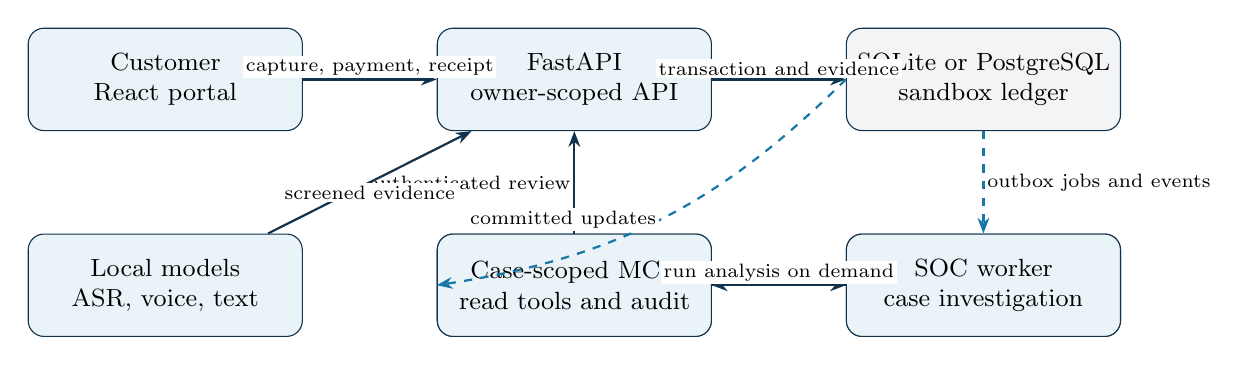
\begin{tikzpicture}[node distance=13mm and 17mm]
\node[box] (customer) {Customer\\React portal};
\node[box,right=of customer] (api) {FastAPI\\owner-scoped API};
\node[store,right=of api] (db) {SQLite or PostgreSQL\\sandbox ledger};
\node[human,below=of api] (analyst) {Analyst\\React workspace};
\node[box,right=of analyst] (gemini) {Optional Gemini\\five-stage analysis};
\node[box,below=of db] (worker) {SOC worker\\case investigation};
\node[box,left=of worker] (mcp) {Case-scoped MCP\\read tools and audit};
\node[box,below=of customer] (models) {Local models\\ASR, voice, text};
\draw[flow] (customer)--node[label,above]{capture, payment, receipt}(api);
\draw[flow] (api)--node[label,above]{transaction and evidence}(db);
\draw[flow] (analyst)--node[label,left]{authenticated review}(api);
\draw[asyncflow] (db)--node[label,right]{outbox jobs and events}(worker);
\draw[flow] (worker)--(mcp);
\draw[asyncflow] (db.west) to[bend left=18] node[label,left]{committed updates}(analyst.west);
\draw[flow] (analyst)--node[label,above]{run analysis on demand}(gemini);
\draw[flow] (models)--node[label,below]{screened evidence}(api);
\end{tikzpicture}
\end{center}
Solid arrows indicate request-time or direct tool interactions. Dashed arrows indicate queued work or delivery from committed records.

\section{End-to-end customer payment flow}
\begin{enumerate}
\item \textbf{Create a session and sandbox account.} The browser receives an owner token. Account and contact records are scoped to that owner.
\item \textbf{Save a beneficiary.} The backend normalizes the reference and associates it with a sandbox counterparty. If the reference matches an existing sandbox account, the relationship can be linked.
\item \textbf{Obtain explicit voice-screening consent.} The browser captures microphone audio as mono 16 kHz PCM using an AudioWorklet, or decodes and resamples a selected clip to the same format. It streams bounded chunks to the API.
\item \textbf{Validate capture.} The backend measures duration, voiced activity, level, and clipping. Unusable recordings are rejected before a payment is created. Raw PCM stays in bounded memory or the configured shared audio cache and is discarded after screening.
\item \textbf{Run inference.} Whisper produces a transcript. AASIST-L or the configured voice provider produces a review-only authenticity result. Scam-detection evaluates spoken text and a supplied typed remark. Missing, unsupported, or failed model results remain explicitly unavailable or inconclusive.
\item \textbf{Build relationship evidence.} A bounded NetworkX graph uses settled sandbox history. The proposed transfer is represented separately from settled transfers.
\item \textbf{Apply deterministic gateway policy.} Active restrictions can block. Eligible corroborated evidence can hold. Other concerns or incomplete evidence can require step-up verification. Otherwise the payment is allowed. Policy version is recorded with the decision.
\item \textbf{Write atomically.} A single SQL transaction records the payment, risk assessment, evidence, and either settlement or case, events, and outbox work. The idempotency key makes identical retries replay the original receipt.
\item \textbf{Return the receipt.} The customer can review status and history. Verification or a later analyst decision updates the authenticated receipt.
\end{enumerate}

\subsection{Policy outcomes}
\begin{tabularx}{\linewidth}{@{}lX@{}}
\toprule
Outcome & Meaning in the sandbox \\
\midrule
ALLOW & The gateway records a settlement in the same database transaction. \\
STEP\_UP & Additional verification is required. The payment is not treated as settled until that step completes. \\
HOLD & The case requires analyst attention and settlement is withheld. \\
BLOCK & An active restriction or other blocking condition prevents the transfer. \\
\bottomrule
\end{tabularx}

\section{Transaction Risk Monitor}
Every newly submitted payment gets one deterministic assessment stored against its payment ID. An identical replay does not create another assessment. The assessment includes score from 0 to 100, band, alert threshold result, contributing signal codes and points, explanations, historical baseline, and suggested analyst action. It is a prioritization aid, not a calibrated fraud probability and does not itself change gateway disposition.

\subsection{Inputs and current rules}
\begin{longtable}{@{}p{0.24\linewidth}p{0.31\linewidth}p{0.36\linewidth}@{}}
\toprule
Input or signal & Current check & Evidence shown \\
\midrule
\endhead
Settled account history & Up to 90 days, maximum 500 rows. At least 10 historical samples are needed for amount and timing comparisons. & Sample count, average, 90th percentile, and example payment IDs. \\
Amount outlier & Amount is at least three times the historical average and exceeds the historical 90th percentile. & Current amount and historical comparison. \\
New high-value beneficiary & Outgoing transfer, no prior settled transfer from this account to this counterparty, beneficiary added within seven days, amount at least \inr 50,000. & Beneficiary ID and added time. \\
Frequency & Counts all submissions in the last 5, 30, 60, and 1,440 minutes. Thresholds are 4, 8, 12, and 24. & Every breached window, count, and threshold. \\
Unusual time & For accounts with enough history, a high-value transfer at least \inr 50,000 falls into a four-hour local-time period used by at most five percent of historical samples. & Time period, sample count, and configured UTC offset. \\
Outgoing surge & Recent settled outgoing value plus this payment reaches at least three times the estimated historical daily amount and at least \inr 50,000. & Recent total, historical daily estimate, and 24-hour window. \\
Previously flagged party & Active restriction or a prior high-priority case matching the account or counterparty. & Account and counterparty identifiers. \\
\bottomrule
\end{longtable}
Weights are 20, 20, 15, 10, 15, and 20 points in the order above. Scores are capped at 100. Bands are LOW (0--24), MEDIUM (25--49), HIGH (50--74), and CRITICAL (75--100). Scores of 50 or more are marked as risk alerts. The current configuration is defined in code and displayed read-only in the workspace.

\subsection{Where it appears}
Authenticated routes under \texttt{/api/v2/analyst/intelligence} provide risk listing and detail, AML listing and detail, review updates, and configuration reads. The Risk Monitor page filters by band, account, beneficiary, date, amount, and alert status. Case Investigator views also show the stored score and evidence. A new assessment is created on payment submission. Existing old payments are not automatically assessed retroactively.

\section{AML Monitoring}
AML monitoring is a separate pattern detector. The current implemented pattern is \textbf{COMMON\_BENEFICIARY\_PATTERN}. On each sandbox settlement, TRINETRA checks a rolling seven-day window for at least four settled outgoing transfers to the same recipient from at least three distinct sender accounts. Incoming requests are interpreted according to their settled ledger direction. In the case where the counterparty links to a sandbox recipient account, transfers from other customers to that account are included as inbound activity.

An alert stores a unique ID, pattern, recipient key, scope, severity, creation and window timestamps, configuration version, explanation, counts, total amount, and bounded supporting payment records. An association table links alert evidence to payments. A unique scope, pattern, recipient, and window end prevents duplicate alerts for the same scan boundary. Further alerts may appear after the previous window expires and a new qualifying pattern is observed. Status starts at NEW. An authenticated analyst can transition it to UNDER\_REVIEW, ESCALATED, RESOLVED, or FALSE\_POSITIVE with a required note. Each status change is retained in the AML review audit table.

The current implementation detects common-beneficiary activity only. Structuring, cumulative deposits, and rapid fund movement described in the source product prompt are not implemented. An alert is a reason to investigate, not a determination of laundering.

\section{Case investigation and analyst workflow}
\subsection{SOC worker workflow}
A payment that needs review creates a case. Case evidence includes measured capture quality, transcript when available, voice and text observations, graph snapshot, and policy reasons. A transactional outbox job lets background workers process the case after commit. Workers use leases, retries, and case-version fencing so expired or stale jobs do not overwrite newer case state.

The five SOC stages have bounded MCP access:
\begin{description}[style=nextline,leftmargin=27mm]
\item[Triage] Read case summary and bounded history.
\item[Investigator] Read capture and model evidence, recipient graph, and similar closed cases.
\item[Decision] Record a proposal based on case evidence.
\item[Monitor] Schedule and update recipient watches.
\item[Reporter] Record the rule-based case report and investigation metrics.
\end{description}
The worker's investigation report is deterministic and evidence-linked. It is separate from the optional Gemini workspace analysis.

\subsection{Gemini analyst workflow}
A signed-in analyst can request analysis for the current case version. The backend constructs sanitized facts and runs five sequential LangGraph stages: Triage, Investigator, Decision, Monitor, and Reporter. Each stage receives a role-specific subset of facts and prior findings. Gemini produces structured findings with cited evidence references. The analyst may record a disposition and note. For an eligible incoming request, verification requires a completed analysis for the current case version and an authenticated analyst action. That action settles the sandbox transfer and updates the customer receipt. Gemini recommendations cannot execute gateway or ledger actions directly.

When configured, LangSmith tracing records workflow runs. Tracing can be disabled. Secrets, voice audio, customer names, account references, raw transcript, and remarks should not be included in tracing payloads.

\section{Investigator and Monitor views}
The Investigator stage displays the recipient network from the stored bounded graph, with settled connections and the transfer under review. It also displays capture levels and quality measurements over time, plus any model score windows. Tables and accessible labels accompany the graph.

The Monitor stage displays the actual scheduled watch: status, next check, horizon, completed checks, and latest check result. Case history events indicate whether new activity reopened a case. This system watch is distinct from a Gemini suggested follow-up.

\section{Major components}
\begin{longtable}{@{}p{0.31\linewidth}p{0.61\linewidth}@{}}
\toprule
Component & Responsibility \\
\midrule
\endhead
React customer portal & Onboarding, saved contacts, voice consent and capture, payment requests, receipts, history. \\
React analyst workspace & Case queue and details, screening evidence, five-stage findings, verification, Risk Monitor, AML Monitoring, Risk Configuration. \\
FastAPI & Owner and analyst APIs, request validation, authentication, case APIs, model listing, WebSocket stream, MCP endpoint. \\
Customer service & Capture lifecycle, payment idempotency, policy inputs, atomic payment and evidence storage, verification. \\
Inference runtime & Manifest and checksum validation, Whisper ASR, AASIST-L ONNX, Scam-detection text model, optional external voice provider. \\
Graph service & Bounded recipient relationship graph built from settled history. \\
Risk and AML service & One-time deterministic payment risk assessment and settlement-triggered common-beneficiary monitoring. \\
Database layer & SQLite default, PostgreSQL concurrent profile, schema migration, transaction wrapper, locking and bounded retries. \\
SOC worker & Outbox handling, investigation, proposals, scheduled watches, case reports. \\
MCP service & Case-scoped JSON-RPC tools, role allow-lists, input validation, redacted audit. The stdio MCP offers read-only analyst tools. \\
Actions service & Version checks, eligibility, action tiers, kill switch, rate limiting, command replay protection. \\
Event service & Transactional event records, outbox, commit-ordered delivery cursor, optional Redis job hints. \\
\bottomrule
\end{longtable}

\section{Data architecture}
\begin{center}
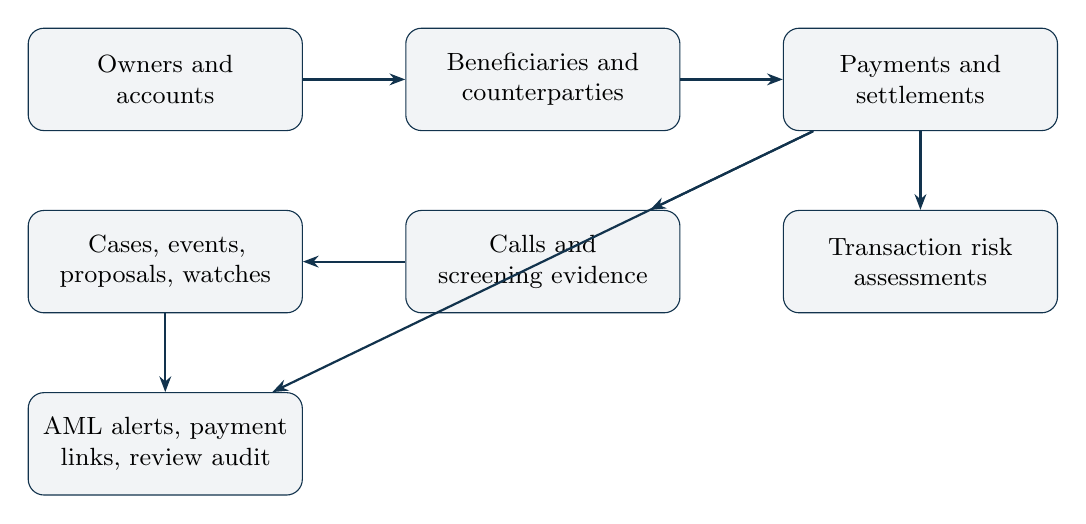
\begin{tikzpicture}[node distance=10mm and 13mm]
\node[store] (owners) {Owners and\\accounts};
\node[store,right=of owners] (benef) {Beneficiaries and\\counterparties};
\node[store,right=of benef] (payments) {Payments and\\settlements};
\node[store,below=of payments] (risk) {Transaction risk\\assessments};
\node[store,left=of risk] (evidence) {Calls and\\screening evidence};
\node[store,left=of evidence] (cases) {Cases, events,\\proposals, watches};
\node[store,below=of cases] (aml) {AML alerts, payment\\links, review audit};
\draw[flow] (owners)--(benef);
\draw[flow] (benef)--(payments);
\draw[flow] (payments)--(risk);
\draw[flow] (payments)--(evidence);
\draw[flow] (evidence)--(cases);
\draw[flow] (cases)--(aml);
\draw[flow] (payments)--(aml);
\end{tikzpicture}
\end{center}
Payments and settlements are the source records for screening, risk history, graph edges, and AML patterns. Model outputs and measurements are evidence records with model ID, revision, status, score, review-only flag, and payload where applicable. Cases link evidence and actions to a versioned investigation trail. AML associations link each alert to its supporting payment IDs. All user-visible analyst queries enforce the configured scope.

\section{Security, privacy, and reliability}
\begin{itemize}
\item Customer sessions are owner scoped. Analyst sessions use signed, expiring tokens. Analyst workspace passwords are configured through the environment or generated for the local workspace.
\item Raw voice is temporary. Only measured quality and inference evidence are persisted. Unsupported, unavailable, and inconclusive outputs remain visible as such.
\item Database writes use transactions. Idempotency keys protect payment retries. Unique constraints protect settlements, jobs, and alert associations. PostgreSQL row locks and advisory locks coordinate concurrent actions.
\item The outbox is authoritative for background work. Workers claim jobs with leases and verify case versions before committing results. Delivery cursors assign order after transaction commits.
\item MCP tools are case scoped, role limited, and audited. Actions check the expected case version, eligibility, configured tier, and kill switch.
\item Inference concurrency and timeouts are bounded. Model artifacts are local and checksum checked. Setting \texttt{HF\_HUB\_OFFLINE=1} allows offline loading after installation.
\item SQLite is suitable for a single-host demonstration. Multi-process API deployments require PostgreSQL and a shared audio cache when audio must move between processes. Redis is optional for job hints and can provide the shared audio cache.
\end{itemize}
\textbf{Model limitation:} model scores are review signals and remain non-enforcing. AASIST-L is diagnostic because evaluation has shown false positives. A model score is not a probability that fraud occurred and does not identify a speaker.

\section{Deployment shape and configuration}
For local use, \texttt{scripts/start.sh} builds the React app and serves it with FastAPI on port 8000. \texttt{scripts/dev.sh} runs FastAPI on port 8000 and Vite on port 5173. SQLite is the default database. For concurrent deployment, PostgreSQL provides transactional coordination. Workers can run in-process or as separate processes. Redis is optional for queue hints and required as a shared PCM cache only when multiple API processes share voice capture.

Key settings include \texttt{TRINETRA\_DATABASE\_URL}, \texttt{TRINETRA\_DATA\_DIR}, \texttt{TRINETRA\_MODEL\_DIR}, \texttt{TRINETRA\_WORKERS}, \texttt{TRINETRA\_VOICE\_PROVIDER}, \texttt{TRINETRA\_AUDIO\_CACHE\_URL}, \texttt{TRINETRA\_SOC\_TIER}, and \texttt{TRINETRA\_SOC\_KILL\_SWITCH}. Gemini requires \texttt{GOOGLE\_API\_KEY} or \texttt{GEMINI\_API\_KEY} and is not required for customer payment screening. Environment values inherited by a process can take precedence over an env file, so deployment configuration should be checked as a whole.

\section{Representative API map}
\begin{tabularx}{\linewidth}{@{}lX@{}}
\toprule
Route & Use \\
\midrule
\texttt{/api/v2/session}, \texttt{/accounts}, \texttt{/beneficiaries} & Customer session and sandbox setup. \\
\texttt{/api/v2/calls} & Consent-bound voice capture, PCM chunks, finish and measured result. \\
\texttt{/api/v2/payments} & Outgoing transfer submission, idempotency and receipt access. \\
\texttt{/api/v2/payment-requests} & Incoming sandbox money request. \\
\texttt{/api/v2/analyst/cases} & Signed-in analyst queue and case details. \\
\texttt{/api/v2/analyst/cases/\{id\}/analysis} & Run current-version Gemini analysis. \\
\texttt{/api/v2/analyst/intelligence/risk} & Risk list and payment risk detail. \\
\texttt{/api/v2/analyst/intelligence/aml} & AML alert list, detail, and audited status review. \\
\texttt{/api/v2/analyst/intelligence/config} & Read current risk and AML thresholds. \\
\texttt{/api/v2/soc/mcp}, stdio MCP & Authenticated HTTP MCP or host-side read-only stdio MCP. \\
\texttt{/api/v2/soc/stream} & Authenticated case update WebSocket. \\
\texttt{/api/health} & Backend health check and database type. \\
\bottomrule
\end{tabularx}

\section{Demonstration walkthrough}
\begin{enumerate}
\item Create a sandbox customer and save a contact. Record a usable voice sample with consent, then submit a payment.
\item Show the receipt and open the analyst case. Inspect the policy reasons and evidence provenance.
\item Run Gemini analysis when the key is configured. Walk through Triage, Investigator, Decision, Monitor, and Reporter findings. Use the Investigator graph and voice timeline, then show the persisted Monitor watch.
\item Open Transaction Risk Monitor. A newly submitted payment already has a stored assessment. Build at least ten settled account samples to demonstrate history-based amount and timing comparisons.
\item Demonstrate a common-beneficiary AML alert using four settled sandbox transfers from at least three sender accounts to the same recipient within seven days. Open the supporting transfer list and record an analyst review note.
\end{enumerate}
Demo records should be created through the normal sandbox payment flow. The risk monitor does not retrospectively score old payments. AML alerts require settled transfers. A payment requiring verification is not counted as settled until verified.

\section{Quality checks}
The repository includes backend unit, integration, concurrency, migration, and model tests, frontend unit and type checks, and browser walkthroughs. The full test command is \texttt{scripts/test-all.sh}; live PostgreSQL coverage is enabled with \texttt{TRINETRA\_TEST\_PG\_URL}. Model inference tests require the downloaded, pinned local checkpoints. Browser tests use isolated databases and exercise customer and analyst journeys.

\section{Source map}
\begin{tabularx}{\linewidth}{@{}lX@{}}
\toprule
Path & Main responsibility \\
\midrule
\texttt{backend/app/main.py}, \texttt{api.py}, \texttt{auth.py} & Application startup, HTTP routes, and authentication. \\
\texttt{backend/app/customer.py}, \texttt{policy.py}, \texttt{inference.py} & Payment lifecycle, gateway rules, voice and text inference. \\
\texttt{backend/app/intelligence.py} & Transaction risk scoring and common-beneficiary AML scan. \\
\texttt{backend/app/db.py}, \texttt{events.py}, \texttt{graph.py} & Persistent schema, event/outbox delivery, recipient graph. \\
\texttt{backend/app/soc/} & Worker, MCP tools, case views, and guarded actions. \\
\texttt{backend/app/analyst/} & Analyst API, Gemini workflow, risk and AML endpoints. \\
\texttt{frontend/src/customer/} & Customer-facing portal. \\
\texttt{frontend/src/analyst/} & Analyst, investigation, risk, and AML interfaces. \\
\texttt{frontend/src/soc/} & Shared SOC views, charts, network graph, and streaming client. \\
\bottomrule
\end{tabularx}

\section{Terms}
\begin{description}[style=nextline,leftmargin=28mm]
\item[Gateway] Backend component that screens a submitted payment and applies the deterministic policy.
\item[Evidence] A stored observation, such as capture measurements, transcript, model result, or graph snapshot.
\item[Outbox] Database-backed queue written in the same transaction as a case, so committed work is not lost between services.
\item[Idempotency] Replaying the same request key and contents returns the existing result instead of creating a second payment.
\item[Step-up] Additional verification before a sandbox payment can settle.
\item[Review-only model signal] Model result available to help analysts, without authority to force a policy outcome.
\item[MCP] Model Context Protocol. Here it provides constrained, auditable tools for reading case evidence and recording selected workflow operations.
\item[Settlement] A ledger record marking a sandbox payment as completed.
\end{description}

\vfill
\begin{center}\small\textcolor{navy}{TRINETRA is a sandbox demonstration system. Its scoring and AML signals are explainable review aids, not determinations of criminal conduct or real-world creditworthiness.}\end{center}
\end{document}
